\begin{figure*}[!tb]
	\centering
	\begin{subfigure}[b]{\columnwidth}
		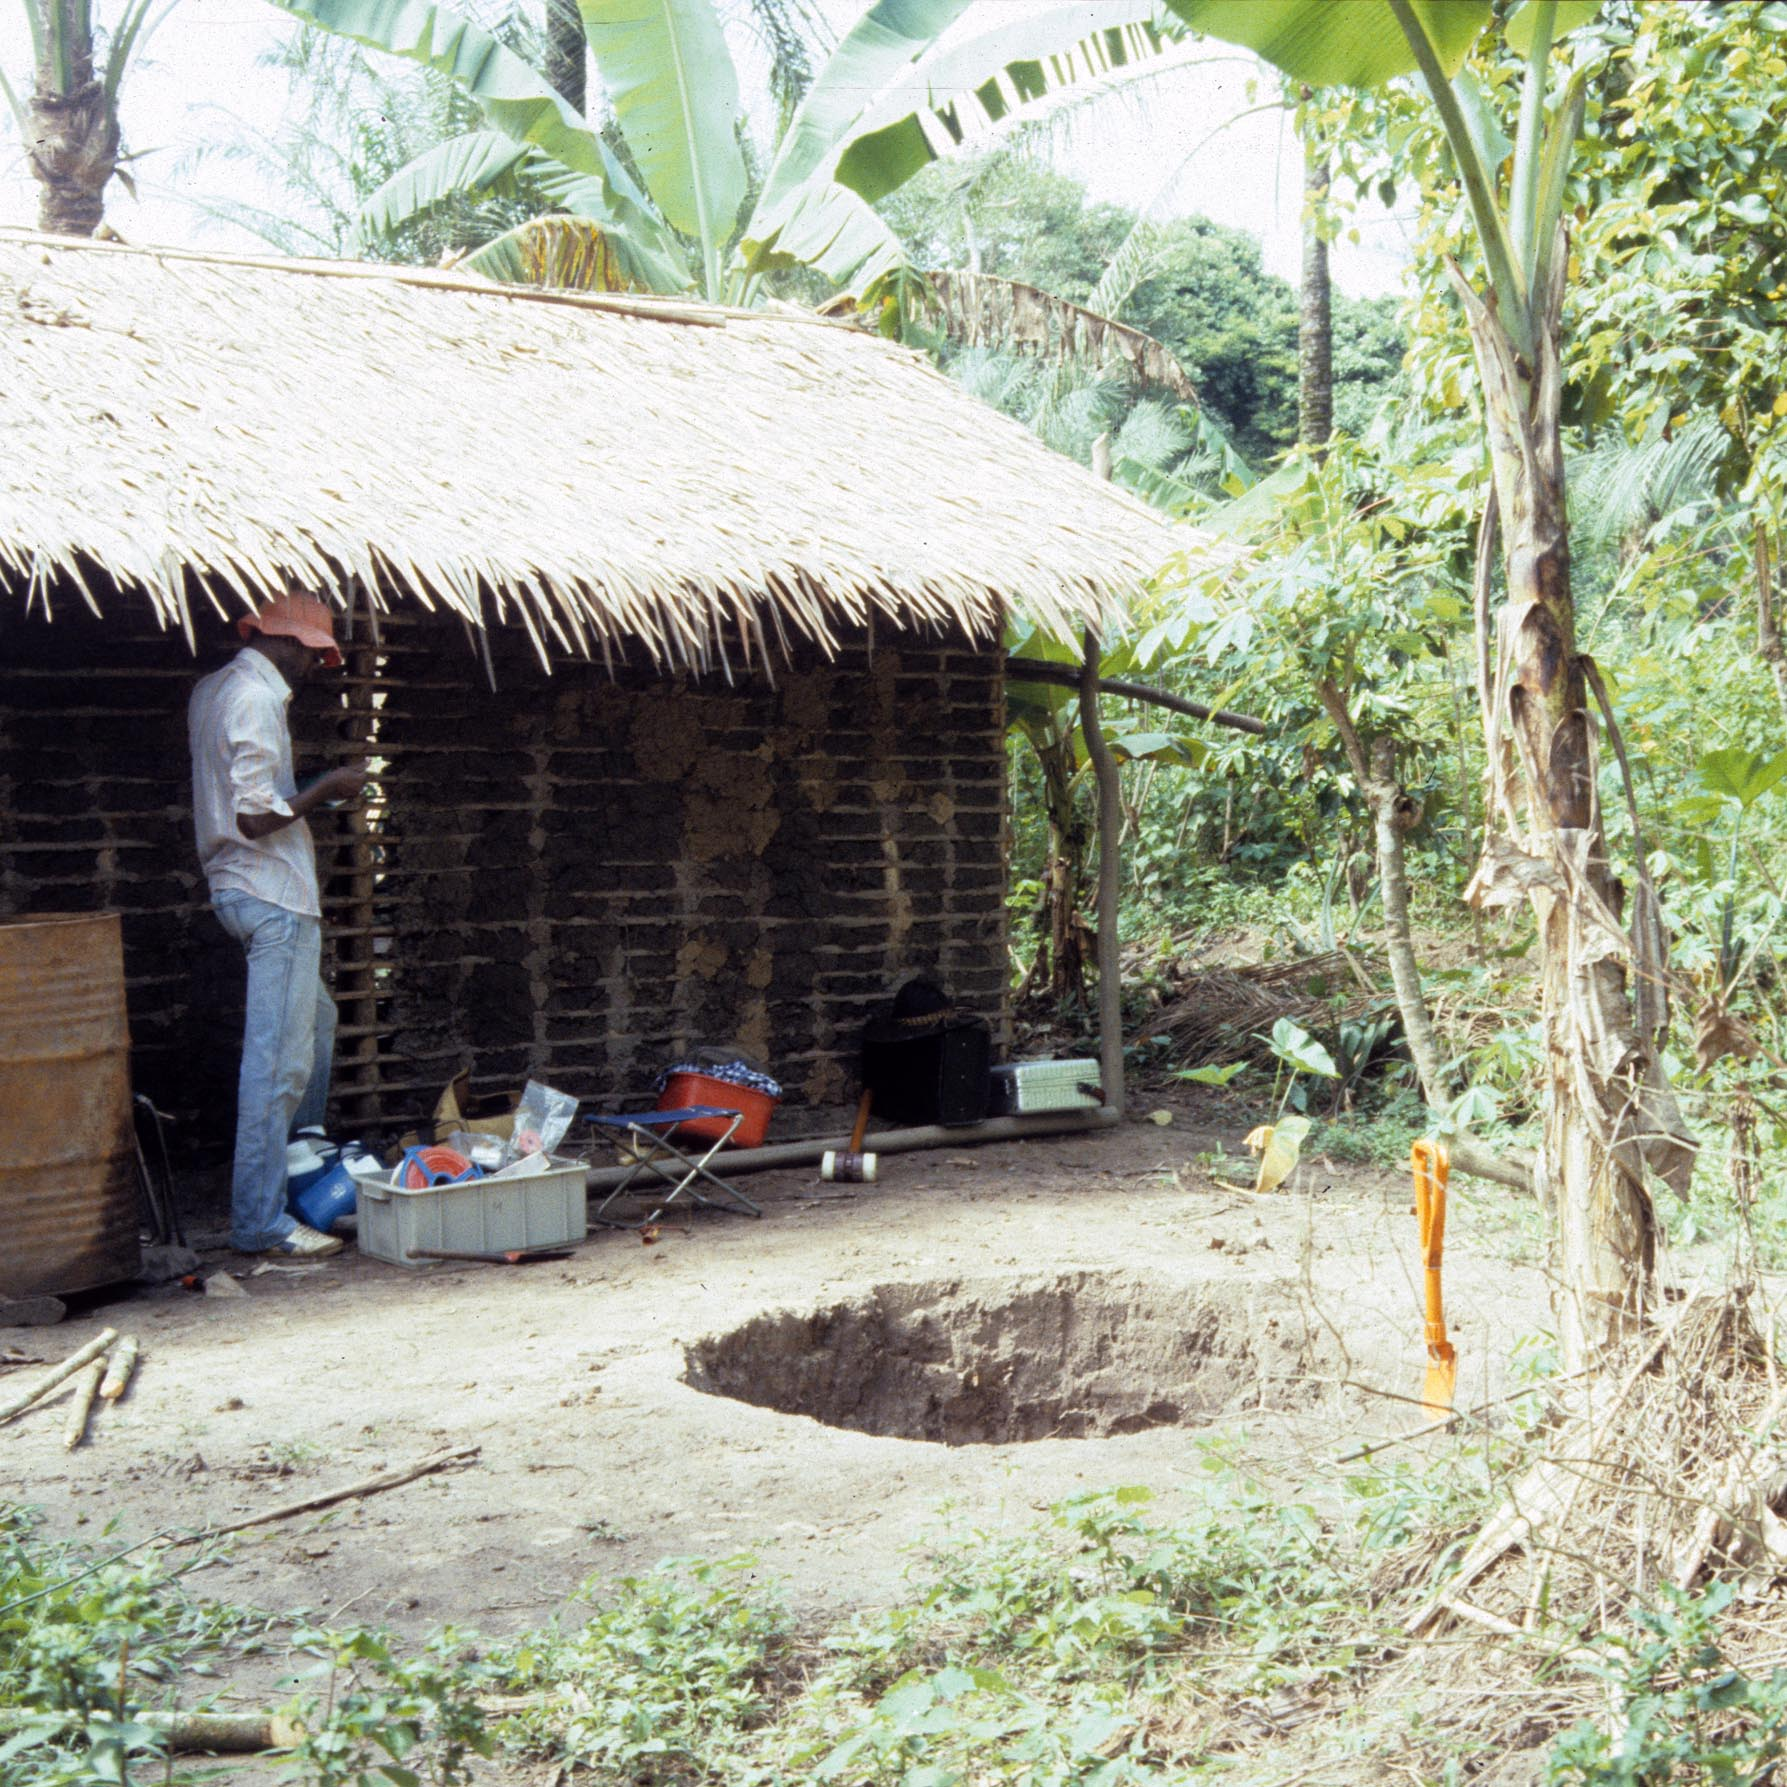
\includegraphics[width = \textwidth]{fig/BBS87-2_E87-02-17.jpg}
		\caption{Überblick über die Grabungsstelle (Foto: M. K. H. Eggert, 1987)}
		\label{fig:BBS87-2_GrubeVorGrabung}
	\end{subfigure}\hfill
	\begin{subfigure}[b]{\columnwidth}
		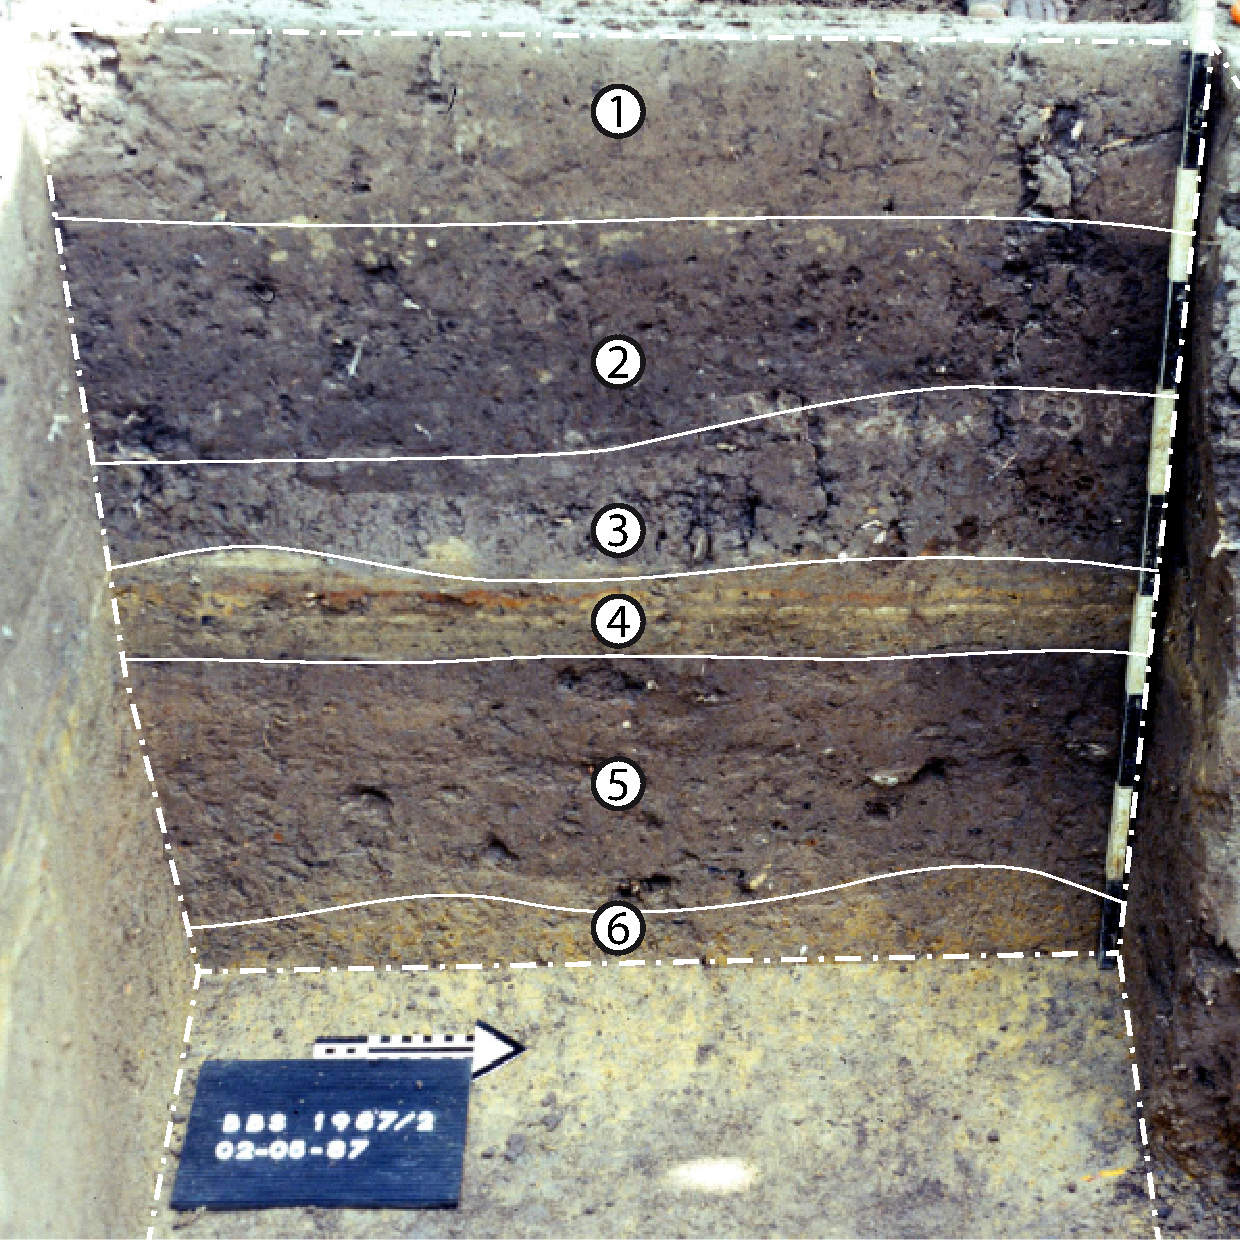
\includegraphics[width = \textwidth]{fig/BBS87-2_H87-01-5.pdf}
		\caption{Kontrollprofil (Foto: H. Holsten, 1987)}
		\label{fig:BBS87-2_OstProfil}
	\end{subfigure}
	\caption{BBS 87/2: Grabungsstelle vor der Untersuchung von Nordwesten (\textbf{A}) und das Kontrollprofil (Ostprofil des Schnitts) vor der Grabung (\textbf{B}).}
	\label{fig:BBS87-2_GrubeVorGrabung_OstProfil}
\end{figure*}

\section*{\begin{tabular*}{\linewidth}{@{}l @{\extracolsep{\fill}} r@{}}
Nr.~7 & BBS~87/2\\
\end{tabular*} 
}

\textsf{\textbf{Bobusa (\mbox{Sangha}; Fpl.~239)}}

\vspace{1em}

\noindent\begin{tabular}{@{}rl@{}}
\textbf{Feldarbeit:} & \textbf{01.05.--05.05.1987 (H. Holsten)} \\ 
\textbf{Abb.:} & \textbf{\ref{fig:BBS87-2_GrubeVorGrabung_OstProfil}--\ref{fig:BBS87-2_Eisenspitze}} \\
\textbf{Tab.:} & \textbf{\ref{tab:BBS87-2_Funde}}\\
\textbf{Taf.:} & \textbf{33.16--33.17} \\ 
\textbf{Lit.:} & \textbf{--} \\ 
\end{tabular}

\paragraph{Grabung und Befunde}\hspace{-.5em}|\hspace{.5em}%
Die Grabung BBS~87/2 erfasste die Befundsituation ausgehend von einer etwa 0,9--1,6\,m großen und knapp 1\,m tiefen Lehmentnahmegrube. Im Anschluss an die Dokumentation des im westlichen Teil der Grube angelegten Profils wurden die fünf sichtbaren Schichten (Abb.~\ref{fig:BBS87-2_GrubeVorGrabung_OstProfil}) in einem 1\,$\times$\,1\,m großen Schnitt ausgegraben.\footnote{Die Abträge zeichnen dabei die im Ost-Profil beobachteten Schichten grob nach, ohne dass explizit nach natürlichen Schichten gegraben wurde.} 

Die Grabung erbrachte drei nahezu fundfreie, dunkel- bis mittelbraune Schichten (1--3), die untereinander nur schwach abgegrenzt waren (Abb.~\ref{fig:BBS87-2_GrubeVorGrabung_OstProfil}). Darauf folgt ein auffällig scharf nach oben abgegrenztes, fein laminiertes, hellgelbes lehmiges \textit{Paket}~4. Schicht~2 überlagert sowohl das lehmige \textit{Paket}~4, als auch die Verfüllung (Schicht~3) einer wannenartigen, 0,1--0,15 m tiefen Eingrabung in das Schicht-Paket~4 (Abb.~\ref{fig:BBS87-2_T76Skizze}--C). Das Schicht-Paket~4 ist mit feinen dunklen, Holzkohle-haltigen sowie roten, angeziegelten Linsen durchzogen. Ein innerhalb des Schicht-Paketes~4 bei etwa 0,6\,m unter der rezenten Oberfläche angelegtes Planum\footnote{Während die Profile gezeichnet und fotografiert wurden (Abb.~\ref{fig:BBS87-2_Profile}), liegen von den angelegten Plana nur einige Fotos und Skizzen vor (Abb.~\ref{fig:BBS87-2_Plana_Foto+Skizzen}).} war stark mit Holzkohle durchsetzt (Abb.~\ref{fig:BBS87-2_T83Skizze}--E). Im östlichen Teil dieses Planums zeigte sich ein sehr flacher, stark rötlich verfärbter Bereich, der als Feuerstelle interpretiert werden kann. 

\begin{figure*}[p]
	\centering
	\begin{subfigure}[t]{.75\textwidth}
		\includegraphics[width = \textwidth, page = 1]{fig/BBS87-2_Plana.pdf}
		\caption{Übersicht über die Profile}
		\label{fig:BBS87-2_SkizzeUebersicht}
	\end{subfigure}
	\begin{subfigure}[t]{.75\columnwidth}
		\includegraphics[width = \columnwidth, page = 2]{fig/BBS87-2_Plana.pdf}
		\caption{Planumsskizze bei zirka 0,5\,m unter Oberfläche (T76)}
		\label{fig:BBS87-2_T76Skizze}
	\end{subfigure}\hspace{1em}
	\begin{subfigure}[t]{.75\columnwidth}
		\includegraphics[width = \columnwidth, page = 3]{fig/BBS87-2_Plana.pdf}
		\caption{Planumsfoto bei zirka 0,5\,m unter Oberfläche (T76; Foto: H. Holsten, 1987)}
		\label{fig:BBS87-2_T76Foto}
		\end{subfigure}
	\begin{subfigure}[t]{.75\columnwidth}
		\includegraphics[width = \columnwidth, page = 4]{fig/BBS87-2_Plana.pdf}
		\caption{Planumsskizze bei zirka 0,6\,m unter Oberfläche (T83)}
		\label{fig:BBS87-2_T83Skizze}
		\end{subfigure}\hspace{1em}
	\begin{subfigure}[t]{.75\columnwidth}
		\includegraphics[width = \columnwidth, page = 5]{fig/BBS87-2_Plana.pdf}
		\caption{Planumsfoto bei zirka 0,6\,m unter Oberfläche (T83; Foto: H. Holsten, 1987)}
		\label{fig:BBS87-2_T83Foto}
		\end{subfigure}
	\begin{subfigure}[t]{.75\columnwidth}
		\includegraphics[width = \columnwidth, page = 6]{fig/BBS87-2_Plana.pdf}
		\caption{Planumsskizze bei zirka 0,7\,m unter Oberfläche (T89)}
		\label{fig:BBS87-2_T89Skizze}
		\end{subfigure}\hspace{1em}
	\begin{subfigure}[t]{.75\columnwidth}
		\mbox{}
	\end{subfigure}
	\caption{BBS 87/2: Skizzen und Fotos der angelegten Zwischenplana.}
	\label{fig:BBS87-2_Plana_Foto+Skizzen}
\end{figure*}

\begin{sidewaysfigure*}[p]
	\centering
	\vspace{8cm}
	\begin{minipage}[t]{\textwidth}
		\includegraphics[width=\textwidth]{fig/BBS87-2_ProfSkizze_kompr.pdf}
		\caption{BBS 87/2: Süd-,West- und Nord-Profile (photogrammetrisch entzerrt) mit Nummerierung der Schichten sowie der engeschnitten Pfostenlöcher A und B (siehe Abb.~\ref{fig:BBS87-2_Plana_Foto+Skizzen}: T89; Fotos: H. Holsten, 1987).}
		\label{fig:BBS87-2_Profile}
	\end{minipage}
\end{sidewaysfigure*}

\begin{table*}[tb]
	\centering
	{\footnotesize \begin{sftabular}{@{}lrrrr@{}}
\toprule
   \textbf{Fundkategorie} &  \textbf{Anzahl} &    \textbf{\%} &  \textbf{Gewicht (kg)} &    \textbf{\%} \\
\midrule
           Eisen &       2 &   1,8 &          0,28 &  22,5 \\
 gebrannter Lehm &      10 &   9,1 &          0,14 &  11,7 \\
         Keramik &      95 &  86,4 &          0,72 &  57,7 \\
          Sonder &       1 &   0,9 &             - &   - \\
           Stein &       2 &   1,8 &          0,10 &   8,1 \\
\bottomrule
\end{sftabular}
}
	\caption{BBS~87/2: Anteil verschiedener Fundmaterialien.}
	\label{tab:BBS87-2_Funde}
\end{table*}

\begin{figure*}[tb]
	\centering
	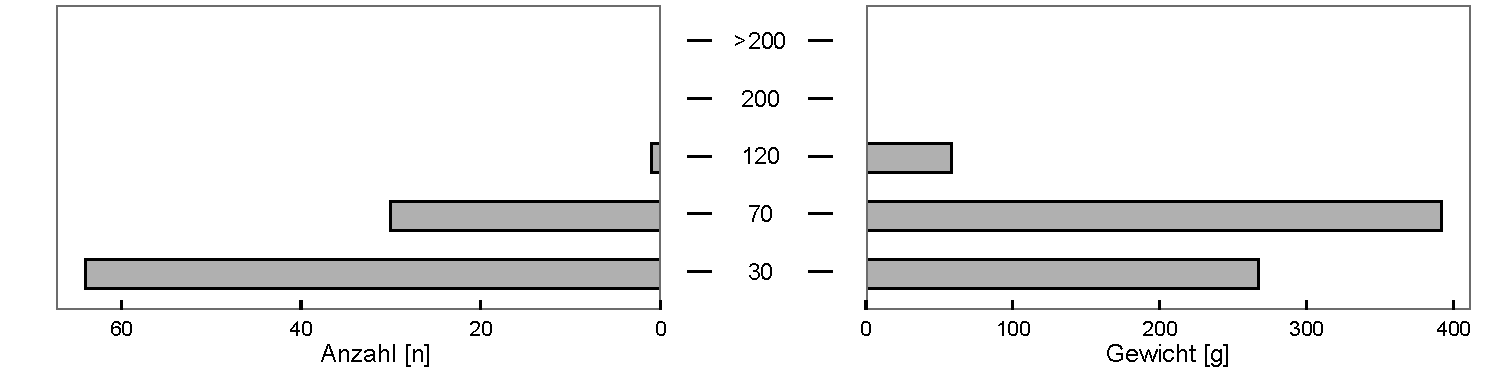
\includegraphics[width=\textwidth]{fig/9-7_BBS87-2_Fragmentierung_2.pdf}
	\caption{BBS~87/2: Fragmentierungsgrad der Scherben  (n~=~95; Größenklassen siehe Anm.~\ref{ftn:Keramik_Fragmentierung}).}
	\label{fig:Fragmenierung_BBS87-2}
\end{figure*}

Bei etwa 0,7\,m unter der Oberfläche (Abb.~\ref{fig:BBS87-2_T89Skizze}) wurde eine grob Nord--Süd-verlaufende Reihe aus fünf Stangenlöchern freigelegt. Die Stangen lagen etwa 0,2--0,3\,m auseinander und hatten einen Durchmesser von 0,6--0,8\,cm. Ihre Verfüllung bestand aus lockerem und dunklerem Substrat. Im Süd-Profil ist ein Pfostenloch (Abb.~\ref{fig:BBS87-2_T89Skizze}, \ref{fig:BBS87-2_Profile}:A) angeschnitten worden. Vor dem West-Profil wurde ein Profilsockel zur Untersuchung eines weiteren Pfostenloches (Abb.~\ref{fig:BBS87-2_T89Skizze}, \ref{fig:BBS87-2_Profile}:B) stehen gelassen. Die Richtung der Pfostenreihe deckt sich mit der Grenze der Schichten~3 und 4 aus dem zweiten Planum (Abb.~\ref{fig:BBS87-2_T76Skizze}--C). Schicht 3, die Verfüllung der wannenartigen, 0,1--0,15\,m mächtigen Vertiefung innerhalb von Schicht~4, teilt die Fläche in zwei Bereiche, deren Grenze sich im Verlauf der Pfostenreihe spiegelt. Dies lässt es naheliegend erscheinen, dass die Wand eines Gebäudes erfasst wurde. Aufgrund des kleines Aufschlusses -- von lediglich 1\,$\times$\,1\,m -- kann nicht sicher gesagt werden, welche der beiden Bereiche die potenzielle \textit{Innen}- beziehungsweise \textit{Außen}-Seite widerspiegelt.\footnote{In Bolondo am Tshuapa sind die Gebäude leicht erhaben auf Plattformen aus Lehm errichtet \parencite[369--376]{Wotzka.1995} . Diese erinnern an den durch Schicht~4 in Bobusa freigelegten Befund. Schicht~3 kann potenziell als wandparalleler, flacher Graben gedeutet werden.}

\noindent Die Grabung erbrachte den folgenden stratigrafischen Befund (Abb.~\ref{fig:BBS87-2_GrubeVorGrabung_OstProfil}; \ref{fig:BBS87-2_Profile}):
\begin{itemize}[leftmargin=*, labelindent=1em, noitemsep, topsep=0pt]
\item [(1)] \textit{Deckschicht}; mittel-/dunkelbraun; keine Funde; \textasciitilde0,15--0,2\,m mächtig
\item [(2)] dunkler als (1); keine Funde; \textasciitilde0,2--0,25\,m mächtig
\item [(3)] mittelbraun, heller als (2) beziehungsweise wie (1); zieht wannenartig in (4); wenige Funde und Holzkohle; \textasciitilde0,15\,m mächtig
\item [(4)] gelber Lehm, durchzogen von roten und dunklen Linsen; an der Basis von Schicht~4 sehr feine tonig-aschige Lagen; im östlichen Teil \textless\,0,1\,m mächtig, im westlichen Teil \textgreater\,0,3\,m mächtig
\item [(5)] mittelbraun; dunkel; homogen; schluffig--tonig; enthält viel Keramik und Holzkohle
\item [(6)] gelber anstehender Lehm
\end{itemize}

\paragraph{Keramik\vspace{.5em}}\mbox{}\\
\begin{tabular}{@{}lrl@{}}
Ausgezählt: & 328\,g & \\ 
Bearbeitet: & 342\,g & (51\,\%) \\ 
Insgesamt: & 670\,g & \\ 
\end{tabular} 

\begin{figure*}[p]
	\centering
	\begin{subfigure}[t]{\textwidth}
		\centering
		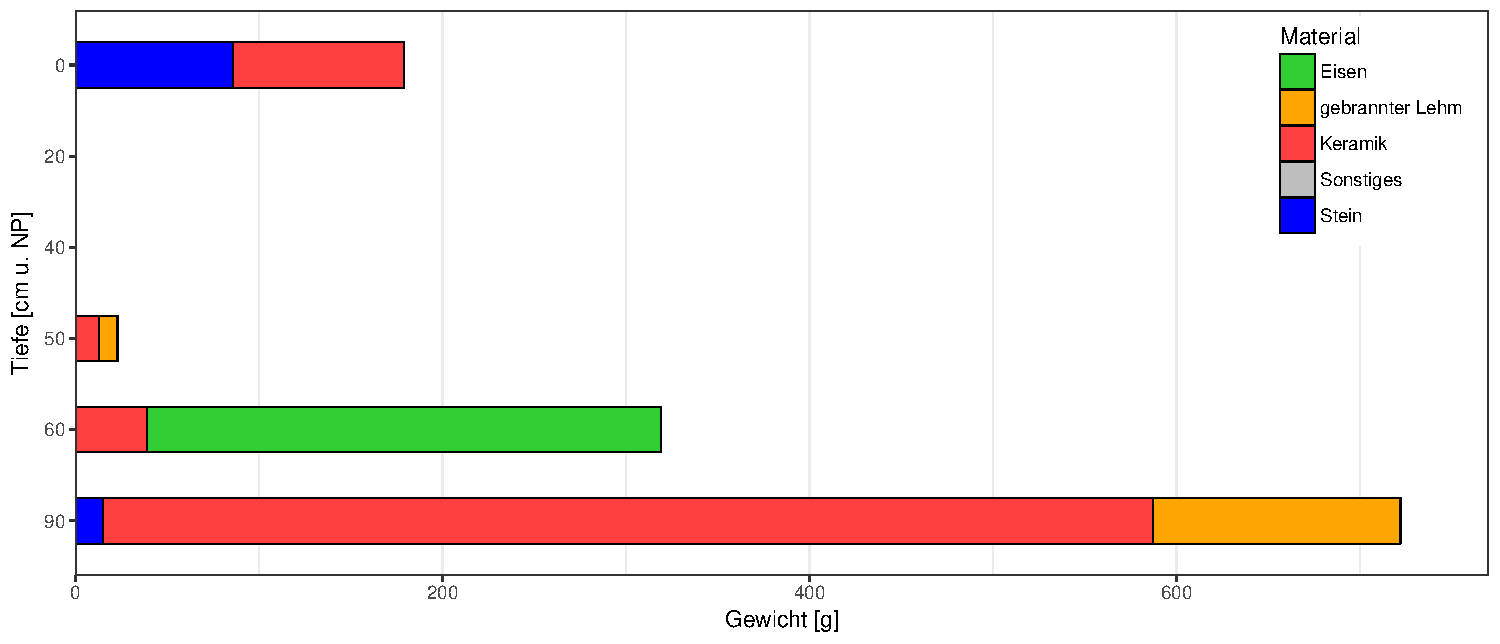
\includegraphics[width=\textwidth]{fig/9-7_BBS87-2_VerteilungFunde_R.pdf}
		\caption{Fundmaterial.\vspace{1em}}
		\label{fig:BBS87-2_VerteilungFunde}
	\end{subfigure}
	\begin{subfigure}[t]{\textwidth}
		\centering
		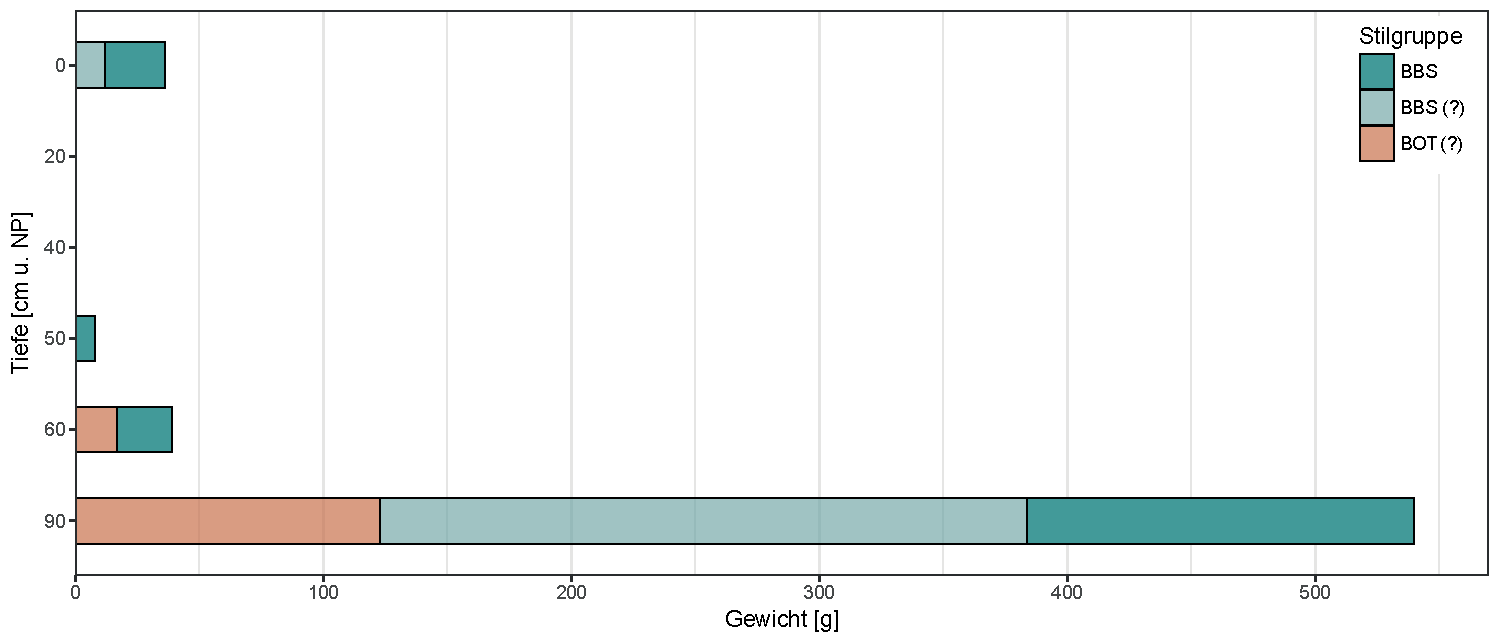
\includegraphics[width=\textwidth]{fig/9-7_BBS87-2_KeramikStilgruppen_R.pdf}
		\caption{Keramische Stilgruppen.\vspace{1em}}
		\label{fig:BBS87-2_VerteilungStilgr}
	\end{subfigure}
	\begin{subfigure}[t]{\textwidth}
		\centering
		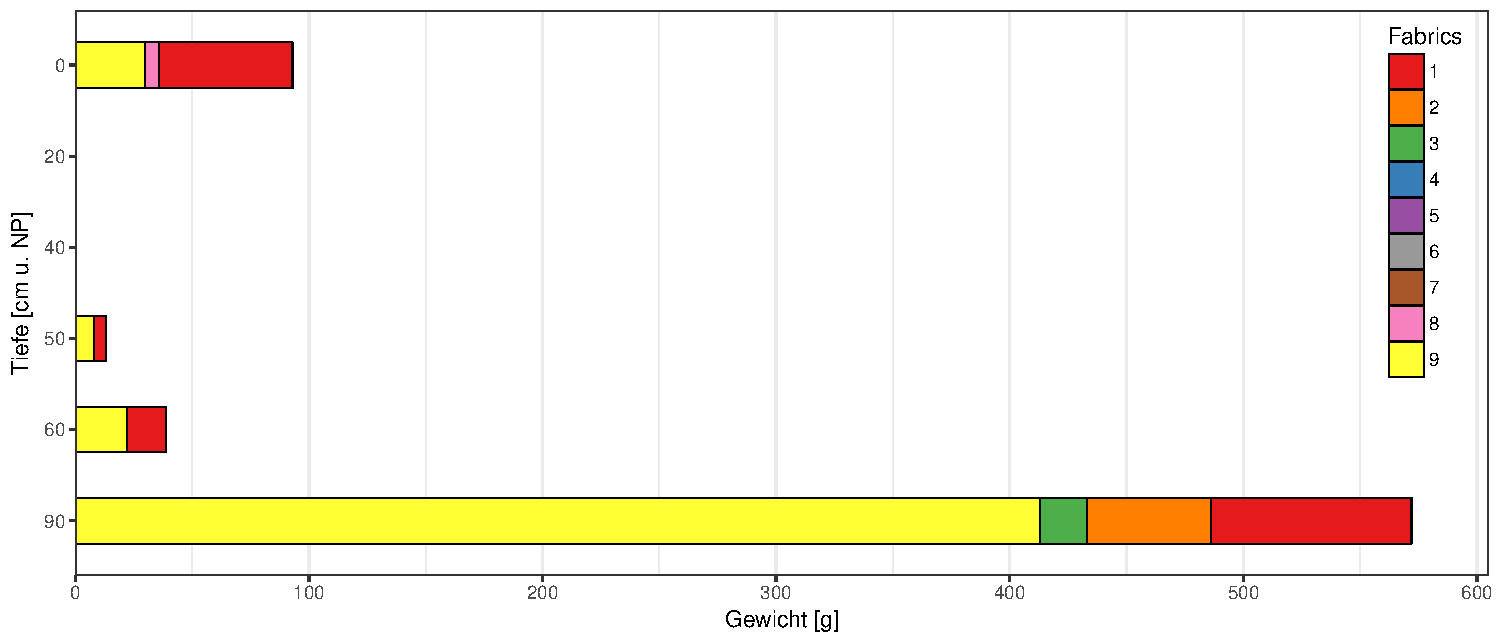
\includegraphics[width=\textwidth]{fig/9-7_BBS87-2_Fabrics_R.pdf}
		\caption{\textit{Fabrics}.}
		\label{fig:BBS87-2_VerteilungFabrics}
	\end{subfigure}
	\caption{BBS 87/2: Verteilung der Fundmaterialien (A), keramischen Stilgruppen (B) und \textit{Fabrics} (C) in den entsprechenden Tiefen der Grabung.}
	\label{fig:BBS87_2_Funde}
\end{figure*}

\vspace{1em}
\noindent Die Keramik aus der Grabung ist stark fragmentiert, Oberflächen der Scherben sind stark erodiert und Bruchkanten deutlich verrundet. Lediglich eine potenziell dem Botendo-Stil (Kap.~\ref{sec:BOT-Gr}) zurechenbare Randscherbe aus Schicht~5 ist größer als 70\,$\times$\,70\,mm. Die übrigen Scherben sind kleiner, wobei Stücke unterhalb von 30\,$\times$\,30\,mm überwiegen (Abb.~\ref{fig:Fragmenierung_BBS87-2}). Häufig sind Fragmente gerade ausbiegender Ränder mit spitzen Mündungen. Ein Teil der Scherben weist zwar formale Ähnlichkeiten zu den Stilen Botendo (Kap.~\ref{sec:BOT-Gr}) sowie Mobaka (Kap.~\ref{sec:MKA-Gr}) auf, unterscheidet sich aber durch regelhafte Schamott-Magerung (Abb.~\ref{fig:BBS87-2_VerteilungFabrics}) deutlich von den Vertretern dieser Stile an anderen Fundstellen. Die Keramik ist nur sehr spärlich verziert. Wenn überhaupt, so lassen sich fast ausschließlich horizontale Rillen (Tab.~\ref{tab:Verzierungselemente}: 02.1; 90\,\%) beobachten. Nur an jeweils einer GE ließ sich \textit{banfwa-nfwa} (Tab.~\ref{tab:Verzierungselemente}: 08) oder ein Winkelband (Tab.~\ref{tab:Verzierungselemente}: 01.6) beobachten.

Vertreter des Botendo-Stils fanden sich in großer Anzahl im Oberflächenmaterial aus dem \textit{elali}\footnote{\label{ftn:elali}Dorfwüstungen werden als \textit{bilali}; im Singular \textit{elali} bezeichnet.} (BBS~87/102), während das wenige Material aus dem Dorf (BBS~87/101) eher den Formen der Bobusa-Gruppe entspricht (Kap.~\ref{sec:BBS-Gr}).

\paragraph{Sonstige Funde}\hspace{-.5em}|\hspace{.5em}%
Im südlichen Teil des Schnitts, direkt an der Grenze von Schicht~3 und 4 fand sich etwa 0,5\,m unter der Oberfläche ein Messingdraht, bei dem es sich höchstwahrscheinlich um ein Stück \textit{Mitako}-Geld\footnote{Siehe R. K. \textcite{Eggert.1980a}.} handeln könnte (Abb.~\ref{fig:BBS87-2_T76Skizze}). Der Draht ist 72\,mm lang und hat einen Durchmesser von 4\,mm.

\begin{Figure}
	\centering
	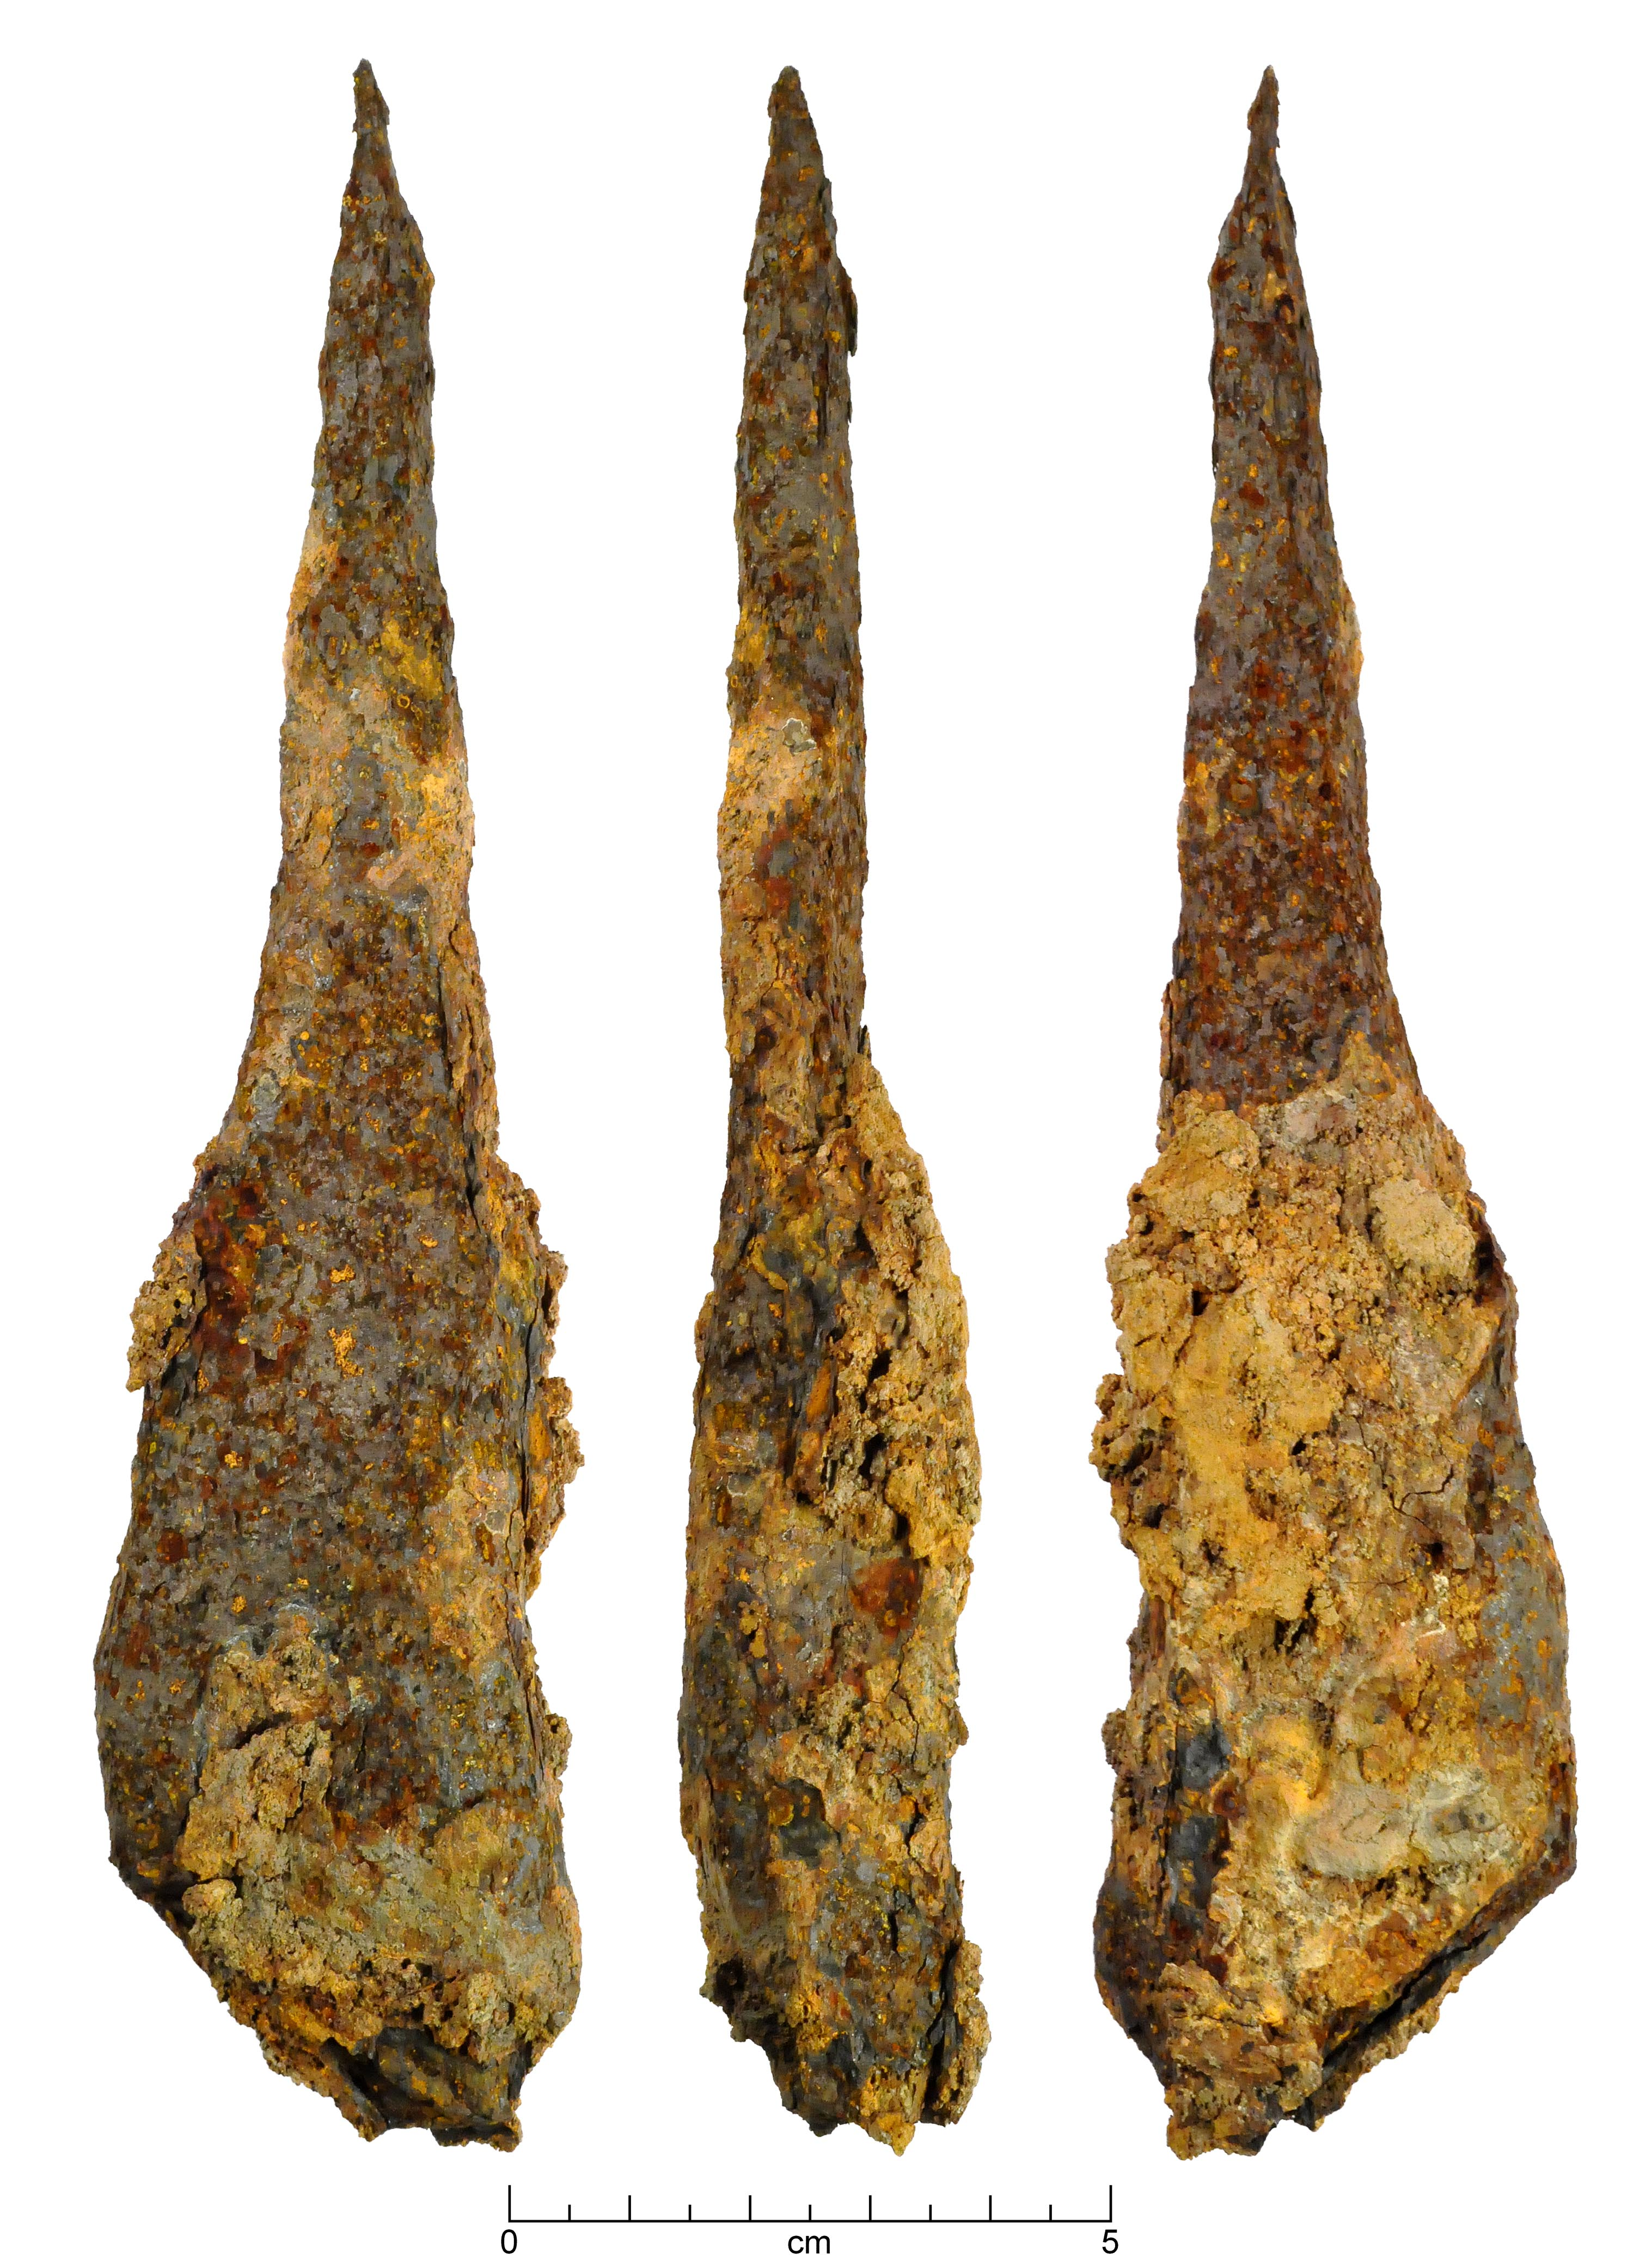
\includegraphics[width=.95\columnwidth]{fig/BBS87-2-4_Eisenspitze.jpg}
	\captionof{figure}{BBS 87/2: Eisenspitze (Foto: D. Seidensticker, 2014)}
	\label{fig:BBS87-2_Eisenspitze}
\end{Figure}

Kurz vor dem Nordprofil fand sich etwa 0,6\,m unter der Oberfläche eine Eisenspitze (Abb.~\ref{fig:BBS87-2_T83Skizze}, \ref{fig:BBS87-2_Eisenspitze}). Sie lag mit der Spitze nach Westen im gelben Lehm der Schicht~4. Die sehr massive Spitze ist 173\,mm lang, 39\,mm breit und 21\,mm hoch und hat einen rechteckigen Querschnitt. Sie weist keine Spuren einer Schäftung auf und aufgrund ihres massiven Charakters kann auch eine potenzielle Funktion als \textit{Barren} nicht ausgeschlossen werden.

\paragraph{Datierung}\hspace{-.5em}|\hspace{.5em}%
Aus der Grabung liegen keine Radiokohlenstoffdatierungen vor. Anhand der keramischen Inventare der einzelnen Schichten und Abträge lassen sich keine chronologischen Schlüsse ableiten. Lediglich die im vierten Abtrag aufgeschlossene Schicht 5 enthielt ein umfangreiches Fundinventar, das sich ausschließlich aus Vertretern der Stilgruppen Bobusa (Kap.~\ref{sec:BBS-Gr}) und Botendo (Kap.~\ref{sec:BOT-Gr}) zusammensetzt (Abb.~\ref{fig:BBS87-2_VerteilungStilgr}). Während die Botendo-Keramik frühestens in das 17.~Jh. n.~Chr. datiert werden kann \parencite[157\,f.]{Wotzka.1995}, lassen sich keine gesicherten Angaben zur Datierung der Bobusa-Keramik machen.

\paragraph{Interpretation}\hspace{-.5em}|\hspace{.5em}%
Der Testschnitt BBS~87/2 deckte unter anderem eine Feuerstelle oberhalb einer etwa 20\,cm mächtigen, fundreichen \textit{Kulturschicht} (Schicht~5) auf. Über der Feuerstelle fand sich ein zirka 0,5\,m mächtiges, fast fundfreies Paket. Des Weiteren wurde eine Nord--Süd-verlaufende Stangenreihe, die potenziell die Wand eines Gebäudes repräsentiert, freigelegt. Die Grenzen einer oberhalb dieser liegenden, flachen Eintiefung verläuft in gleicher Ausrichtung wie die Stangenreihe. Eine Zuordnung der erfassten Stangenlöcher zu einem Wohnhaus lässt sich auf dieser Basis wahrscheinlich machen.\footnote{Die traditionelle Bauweise mit dünnen Stangen und Flechtwerk lässt sich an dem Gebäude direkt neben der Grabung beobachten (Abb.~\ref{fig:BBS87-2_GrubeVorGrabung}).}